\documentclass[times, utf8, diplomski]{fer}
\usepackage{booktabs}
\usepackage{algorithmic}
\usepackage{algorithm}
\usepackage{listings}
\usepackage{longtable}
\usepackage{graphicx}
\usepackage{array}
\usepackage{booktabs}


\begin{document}

% TODO: Navedite broj rada.
\thesisnumber{1720}

% TODO: Navedite naslov rada.
\title{Projektiranje sustava praćenja trajektorije bespilotne letjelice u sustavu globalne vizije}

% TODO: Navedite vaše ime i prezime.
\author{Luka Galović}

\maketitle

% Ispis stranice s napomenom o umetanju izvornika rada. Uklonite naredbu \izvornik ako želite izbaciti tu stranicu.
\izvornik

% Dodavanje zahvale ili prazne stranice. Ako ne želite dodati zahvalu, naredbu ostavite radi prazne stranice.
\zahvala{Svima koji žele naučiti koristiti \LaTeX{}.}

\tableofcontents
% Tu možete staviti popis slika i tablica

\chapter{Uvod}
Ulaskom u novo stoljeće svjedočimo nastavku razvoja, usavršavanja i stvaranja novih tehnologija koja su pomoć u različitim ljudskim aktivnostima. Iako pojam bespilotnih letjelica postoji već dugi niz godina, one su tek u bliskoj prošlosti postale pojam svakodnevnice. Dugi niz godina bespilotne letjelice su se koristile, nažalost, samo u vojnim svrhama zbog čega su stradavali i nedužni civili zbog čega se njihov razvoj držao u tajnosti. Samo saznanje da se koriste u vojsci upućuje na to da je puno vremena i novaca uloženo u njihov razvoj, preciznost, nosivost te izdržljivost.\\
Danas se uz nagli tred upoznavanja s tehnologijama bespilotnih letjelica, kao i digitalnih zapisa i pohranjivanja memorije svakodnevnih događaja namjena korištenja promijenila te su uvedeni novi pojmovi poput \glqq dronovi\grqq --- suvremena riječ koja zapravo opisuje nekoliko vrsta bespilotnih letjelica. Glavna područja njihovih korištenja su: javna sigurnost, zabava, nadzor i inspekcija, informacije, znanost o Zemlji.\\
Korištenje  bespilotnih letjelica, naročito u civilne svrhe, bilježi eksponencijalan rast, kako u pogledu njihovog broja, veličine i težine, tako i u pogledu sve brojnijih mogućnosti njihove primjene \citep{EUR-Lex}.\\
Motiv izrade ovog rada je shvatiti rad bespilotne letjelice te izrada sustava za slijeđenje željene trajektorije. Izazov je kretati se zadanom trajektorijom znajući da postoje razne vanjske smetnje koje utjeću na upravljanje. U teorijskom dijelu će se opisati razvoj, svrha odnosno tipovi bespilotnih letjelica, dok će se detaljnije razraditi njezin model te odrediti matematički model prikladan za sintezu sustava upravljanja. Projektirat će se regulator za slijeđenje reference, uz pretpostavku raspoloživosti informacije o trenutnoj poziciji te orijentaciji. Provjera projektiranog sustava je u simulaciji odnosno eksperimentalno u laboratorijskim uvjetima.

\chapter{Razrada}
\section{Bespilotne letjelice}
Bespilotne letjelice su, najjednostavnije rečeno, letjelice koje su sposobne izvršiti kontinuirani let bez pilota\citep{UAV}. Definiranjem pojma bespilotnih letjelica\footnote{UAV \engl{Unmanned Aerial Vehicle} – opći je pojam koji označava zapravo sve vrste bespilotnih letjelica koje se kolokvijalno najčešće nazivaju dronovima. Pod tim se obično spominju dvije vrste letjelica kojima ne trebaju ljudski piloti, prve su tzv. kvadrikopteri \engl{quadcopter}, letjelice s četiri elise pomoću kojih dron može lebdjeti na mjestu i kretati se u raznim smjerovima. Drugi tip bespilotnih letjelica su izgleda projektila ili zrakoplova kojim se upravlja iz baze i povezani su uglavnom s vojnim operacijama.} nailazi se na bogat izbor objašnjenja jer imaju široku primjenu. \\

\begin{table}[h!]
  \centering
  \begin{tabular}{ | c | m{5cm} | m{5cm} | }
    \hline
    Vrsta & \centering Prednosti & Mane \\ \hline
    \begin{minipage}{.3\textwidth}
      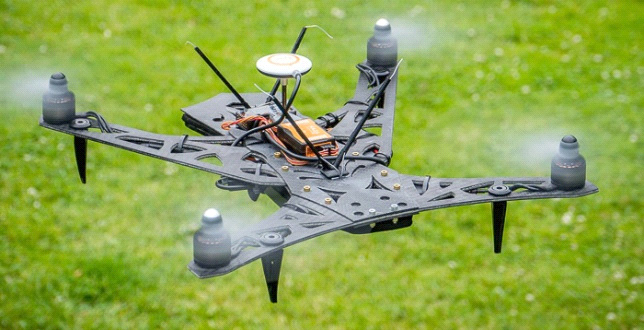
\includegraphics[width=\linewidth, height=60mm]{img/quadcopter.png}
    \end{minipage}
    &
    %\begin{minipage}[t]{5cm}
      \begin{itemize}
        \item Accessibility
        \item Up to date information
        \item Fulfil students needs and wants \ldots
      \end{itemize}
    %\end{minipage}
    & 
    %\begin{minipage}{5cm}
      \begin{itemize}
        \item Accessibility
        \item Up to date information
        \item Fulfil students needs and wants \ldots
      \end{itemize}
    %\end{minipage}
    \\ \hline
  \end{tabular}
  \caption{my.Lboro Analysis}\label{tbl:myLboro}
\end{table}

\chapter{Proba}
Uvod rada. Nakon uvoda dolaze poglavlja u kojima se obrađuje tema.
\section{Odjeljak 1.1}
Tekst o odjeljku
\subsection{Pododjeljak}
\emph{How can we eat?}
Popis fusnota\footnote{Objašnjenja koja se prikazuju
na dnu stranice} nije potreban.
\section{Dodavanje posvete}
\label{sec:posveta}
Za navedeno pogledajte odjeljke \ref{sec:posveta}
\begin{itemize}
	\item prva stavka,
	\item druga stavka,
	\begin{enumerate}
		\item druga razina.
	\end{enumerate}
\end{itemize}

\begin{table}[htb]
\caption{Konstante}
\label{tbl:konstante}
\centering
\begin{tabular}{llr} \toprule
Konstanta & Opis & Vrijednost\\ \midrule
$\pi$ & Pi & 3.14159 \\
$e$ & Eulerov broj & 2.71828 \\
$\varphi$ & Zlatni rez & 1.61803 \\ \bottomrule
\end{tabular}
\end{table}

\begin{figure}[htb]
\centering

\includegraphics[width=5cm]{img/fer_logo.jpg}
\caption{Logo FER-a}
\label{fig:fer-logo}
\end{figure}

‘Prva dama: $\sin^2 \varphi + \cos^2 \varphi = 1$.’ \citep{ungar2002uvod} \cite{oetiket2007lshort}

Dodatak dokumenta \engl{appendix}.

Primjer korištenja enumitem paketa dan je u \citep{collins2008enum}.
\citet{collins2008enum} opisuje korištenje enumitem paketa.
\cite{greenwade93}
Text ... citation: \cite{greenwade93}.

\chapter{Zaključak}
Zaključak.

\bibliographystyle{fer}
\bibliography{literatura}

\begin{sazetak}
Sažetak na hrvatskom jeziku.

\kljucnerijeci{Ključne riječi, odvojene zarezima.}
\end{sazetak}

% TODO: Navedite naslov na engleskom jeziku.
\engtitle{Title}
\begin{abstract}
Abstract.

\keywords{Keywords.}
\end{abstract}

\end{document}
